\documentclass[10pt, aspectratio=169, handout]{beamer}
\usefonttheme{professionalfonts}

\mode<presentation>
{ 
  \usetheme{Berkeley}
  \usecolortheme{beaver}
  \usefonttheme{default}
  \setbeamertemplate{navigation symbols}{} 
  \setbeamertemplate{caption}[numbered]
} 

\setbeamertemplate{footline}{%
  \leavevmode%
  \hbox{% 
    \begin{beamercolorbox}[wd=.85\paperwidth,ht=2.5ex,dp=1ex,left]{author in head/foot}% 
      \usebeamerfont{author in head/foot}Digital Signal Processing, Fall 2025%
    \end{beamercolorbox}% 
    \begin{beamercolorbox}[wd=.15\paperwidth,ht=2.5ex,dp=1ex,right]{date in head/foot}% 
      \hspace*{0.5em}\insertframenumber{} / \inserttotalframenumber\hspace*{0.5em}% 
    \end{beamercolorbox}% 
  }%
  \vskip0pt%
}

\usepackage[english]{babel}
\usepackage[utf8x]{inputenc}
\usepackage{tikz}
\usetikzlibrary{arrows.meta}
\usepackage{pgfplots}
\usepackage{array}
\usepackage{makecell}
\usepackage{verbatim}
\usepackage{graphicx}
\usepackage{subcaption}
\usepackage{amsfonts}
\usepackage{amsmath}
\usepackage{bm}
\usepackage{epstopdf}
\captionsetup{compatibility=false}
\usepackage[absolute,overlay]{textpos}
\usetikzlibrary{calc}
\usetikzlibrary{pgfplots.fillbetween, backgrounds}
\usetikzlibrary{positioning}
\usetikzlibrary{pgfplots.groupplots}
\usetikzlibrary{plotmarks}
\usetikzlibrary{calc}
\usepgfplotslibrary{groupplots}
\pgfplotsset{compat=newest} 

\usepackage{hyperref}
\hypersetup{
    colorlinks=true,
    linkcolor=blue,
    filecolor=magenta,      
    urlcolor=cyan,
}

\title[ECEN 463/863]{Discrete-Time Processing of Continuous-Time Signals}
\author{Department of Electrical and Computer Engineering}
\institute{University of Nebraska-Lincoln}
\date{Fall 2025}

\begin{document}

\begin{frame}
  \titlepage
\end{frame}

\section{Introduction}

\begin{frame}{Overview: Discrete-Time Processing System}
\textbf{General System Architecture}:
\begin{center}
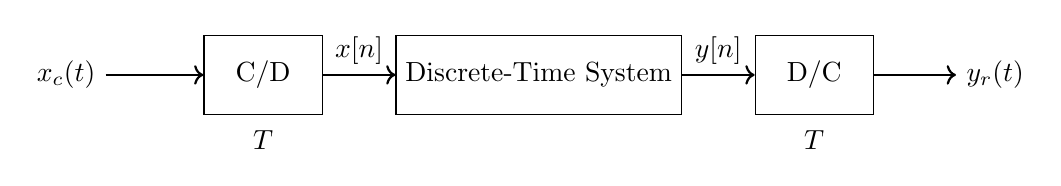
\begin{tikzpicture}
    % Input continuous-time signal
    \node at (-4,0) {$x_c(t)$};
    % First block
    \node[draw, minimum width=1.5cm, minimum height=1cm] (cd) at (-1.5,0) {C/D};
    % Second block
    \node[draw, minimum width=2.2cm, minimum height=1cm] (dt) at (2,0) {Discrete-Time System};
    % Third block
    \node[draw, minimum width=1.5cm, minimum height=1cm] (dc) at (5.5,0) {D/C};
    % Output continuous-time signal
    \node at (7.8,0) {$y_r(t)$};

    % Arrows (use anchors instead of absolute coords)
    \draw[->, thick] (-3.5,0) -- (cd.west);
    \draw[->, thick] (cd.east) -- (dt.west) node[midway, above] {$x[n]$};
    \draw[->, thick] (dt.east) -- (dc.west) node[midway, above] {$y[n]$};
    \draw[->, thick] (dc.east) -- (7.3,0);

    % Sampling period annotations directly under blocks
    \node at (cd.south) [below=2pt] {$T$};
    \node at (dc.south) [below=2pt] {$T$};
\end{tikzpicture}
\end{center}

\vspace{0.3cm}
\textbf{Key Properties}:
\begin{itemize}
    \item Overall system cascade: continuous-time input $\to$ continuous-time output
    \item Equivalent to continuous-time LTI system (under conditions)
    \item Same sampling rate $T$ for C/D and D/C converters
    \item Properties depend on discrete-time system and sampling rate
\end{itemize}
\end{frame}

\begin{frame}{Mathematical Summary: C/D Converter (ADC)}
\textbf{Time Domain - Sample Generation}:
\[
\boxed{x[n] = x_c(nT)}
\]

\vspace{0.3cm}
\textbf{Frequency Domain - Periodic Replication}:
\[
\boxed{X(e^{j\omega}) = \frac{1}{T}\sum_{k=-\infty}^{\infty}X_c\left(j\frac{\omega - 2\pi k}{T}\right)}
\]

\vspace{0.3cm}
\textbf{Key Points}:
\begin{itemize}
    \item DTFT $X(e^{j\omega})$ is periodic with period $2\pi$
    \item Continuous-time frequency: $\Omega$ (rad/s)
    \item Discrete-time frequency: $\omega$ (radians)
    \item Relationship: $\omega = \Omega T$
\end{itemize}
\end{frame}

\begin{frame}{Mathematical Summary: D/C Converter (DAC)}
\textbf{Ideal Bandlimited Interpolation}:
\[
\boxed{y_r(t) = \sum_{n=-\infty}^{\infty}y[n]\frac{\sin[\pi(t-nT)/T]}{\pi(t-nT)/T}}
\]

\vspace{0.3cm}
\textbf{Frequency Domain Relationship}:
\[
\boxed{Y_r(j\Omega) = \begin{cases}
TY(e^{j\Omega T}), & |\Omega| < \pi/T \\
0, & \text{otherwise}
\end{cases}}
\]

\vspace{0.3cm}
\textbf{Interpretation}:
\begin{itemize}
    \item Each sample reconstructed as sinc function
    \item Ideal lowpass filter with cutoff $\Omega_c = \pi/T$
    \item Extracts baseband from periodic spectrum
\end{itemize}
\end{frame}

\section{LTI Processing}

\begin{frame}{Discrete-Time LTI System Processing}
\textbf{LTI System in Frequency Domain}:
\[
Y(e^{j\omega}) = H(e^{j\omega})X(e^{j\omega})
\]

\vspace{0.3cm}
\textbf{Combining with D/C Converter}:
\[
Y_r(j\Omega) = H_r(j\Omega)H(e^{j\Omega T})X(e^{j\Omega T})
\]

\vspace{0.3cm}
\textbf{Using Periodic Replication of $X(e^{j\omega})$}:
\[
Y_r(j\Omega) = H_r(j\Omega)H(e^{j\Omega T})\frac{1}{T}\sum_{k=-\infty}^{\infty}X_c\left(j\left(\Omega - \frac{2\pi k}{T}\right)\right)
\]
\end{frame}

\begin{frame}{Effective Continuous-Time System}
\textbf{Condition}: If $X_c(j\Omega) = 0$ for $|\Omega| \geq \pi/T$ (bandlimited)

\vspace{0.3cm}
Then the ideal reconstruction filter selects only $k=0$ term:
\[
\boxed{Y_r(j\Omega) = H(e^{j\Omega T})X_c(j\Omega), \quad |\Omega| < \pi/T}
\]

\vspace{0.3cm}
\textbf{Effective Frequency Response}:
\[
\boxed{H_{\text{eff}}(j\Omega) = \begin{cases}
H(e^{j\Omega T}), & |\Omega| < \pi/T \\
0, & |\Omega| \geq \pi/T
\end{cases}}
\]

\vspace{0.3cm}
\textbf{Result}: Overall system behaves as continuous-time LTI system
\end{frame}

\begin{frame}{Requirements for LTI Behavior}
\textbf{Two Essential Conditions}:

\vspace{0.3cm}
\textbf{1. Discrete-Time System}:
\begin{itemize}
    \item Must be linear and time-invariant
    \item Characterized by impulse response $h[n]$ or frequency response $H(e^{j\omega})$
\end{itemize}

\vspace{0.3cm}
\textbf{2. Input Signal and Sampling}:
\begin{itemize}
    \item Input $x_c(t)$ must be bandlimited
    \item Sampling rate above Nyquist: $\Omega_s = 2\pi/T > 2\Omega_N$
    \item Aliased components (if any) must be removed by $H(e^{j\omega})$
\end{itemize}

\vspace{0.3cm}
\textbf{Caution}: Time-invariance can fail even with identity system if aliasing occurs
\end{frame}

\section{Example: Ideal Lowpass Filter}

\begin{frame}{Example: Ideal Lowpass Filtering}
\textbf{Discrete-Time Filter}:
\[
H(e^{j\omega}) = \begin{cases}
1, & |\omega| < \omega_c \\
0, & \omega_c < |\omega| \leq \pi
\end{cases}
\]

\begin{center}
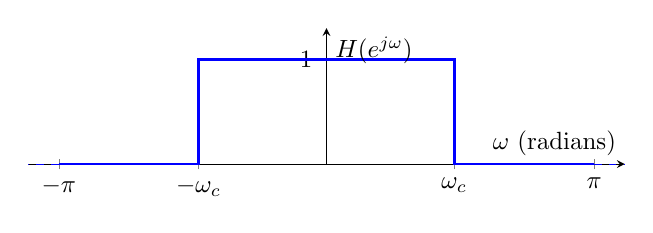
\begin{tikzpicture}[scale=0.9]
    \begin{axis}[
        width=10cm, height=3.5cm,
        xlabel={$\omega$ (radians)},
        ylabel={$H(e^{j\omega})$},
        xmin=-3.5, xmax=3.5,
        ymin=0, ymax=1.3,
        axis lines=middle,
        xtick={-3.14,-1.5,0,1.5,3.14},
        xticklabels={$-\pi$,$-\omega_c$,$0$,$\omega_c$,$\pi$},
        ytick={1},
        yticklabels={$1$}
    ]
    % Main lobe
    \addplot[blue, very thick] coordinates {(-3.14,0) (-1.5,0) (-1.5,1) (1.5,1) (1.5,0) (3.14,0)};
    % Periodic extension indicators
    \draw[blue, dashed] (axis cs:-3.14,0) -- (axis cs:-4.64,0);
    \draw[blue, dashed] (axis cs:-4.64,1) -- (axis cs:-4.64,0);
    \draw[blue, dashed] (axis cs:3.14,0) -- (axis cs:4.64,0);
    \draw[blue, dashed] (axis cs:4.64,1) -- (axis cs:4.64,0);
    \end{axis}
\end{tikzpicture}
\end{center}

\textbf{Note}: Periodic with period $2\pi$
\end{frame}

\begin{frame}{Effective Continuous-Time Lowpass Filter}
\textbf{For bandlimited inputs at/above Nyquist rate}:
\[
H_{\text{eff}}(j\Omega) = \begin{cases}
1, & |\Omega| < \omega_c/T \\
0, & |\Omega| \geq \omega_c/T
\end{cases}
\]

\begin{center}
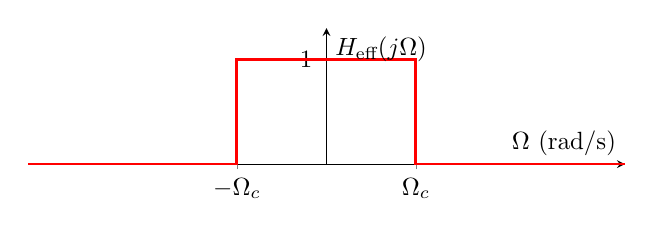
\begin{tikzpicture}[scale=0.9]
    \begin{axis}[
        width=10cm, height=3.5cm,
        xlabel={$\Omega$ (rad/s)},
        ylabel={$H_{\text{eff}}(j\Omega)$},
        xmin=-5, xmax=5,
        ymin=0, ymax=1.3,
        axis lines=middle,
        xtick={-1.5,0,1.5},
        xticklabels={$-\Omega_c$,$0$,$\Omega_c$},
        ytick={1},
        yticklabels={$1$}
    ]
    \addplot[red, very thick] coordinates {(-5,0) (-1.5,0) (-1.5,1) (1.5,1) (1.5,0) (5,0)};
    \end{axis}
\end{tikzpicture}
\end{center}

\textbf{Key Insight}: Cutoff frequency $\Omega_c = \omega_c/T$
\begin{itemize}
    \item Variable $T$ provides tunable continuous-time cutoff
    \item Fixed discrete-time filter, varying sampling rate
\end{itemize}
\end{frame}

\begin{frame}{Frequency Domain Illustration (1/3)}
\textbf{Bandlimited Input Spectrum}:
\begin{center}
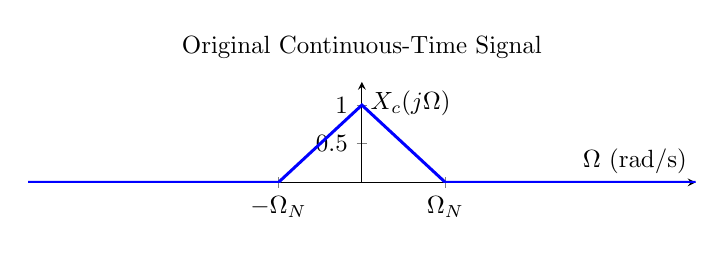
\begin{tikzpicture}[scale=0.9]
    \begin{axis}[
        width=11cm, height=3cm,
        xlabel={$\Omega$ (rad/s)},
        ylabel={$X_c(j\Omega)$},
        xmin=-8, xmax=8,
        ymin=0, ymax=1.3,
        axis lines=middle,
        xtick={-2,0,2},
        xticklabels={$-\Omega_N$,$0$,$\Omega_N$},
        title={Original Continuous-Time Signal}
    ]
    % Triangular spectrum
    \addplot[blue, very thick] coordinates {(-8,0) (-2,0) (0,1) (2,0) (8,0)};
    \end{axis}
\end{tikzpicture}
\end{center}

\textbf{After Sampling - Periodic Replication}:
\begin{center}
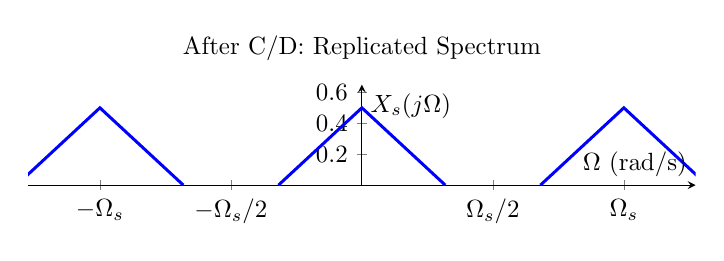
\begin{tikzpicture}[scale=0.9]
    \begin{axis}[
        width=11cm, height=3cm,
        xlabel={$\Omega$ (rad/s)},
        ylabel={$X_s(j\Omega)$},
        xmin=-8, xmax=8,
        ymin=0, ymax=0.65,
        axis lines=middle,
        xtick={-6.28,-3.14,0,3.14,6.28},
        xticklabels={$-\Omega_s$,$-\Omega_s/2$,$0$,$\Omega_s/2$,$\Omega_s$},
        title={After C/D: Replicated Spectrum}
    ]
    % Center copy (scaled by 1/T)
    \addplot[blue, very thick] coordinates {(-2,0) (0,0.5) (2,0)};
    % Left copy
    \addplot[blue, very thick] coordinates {(-8.28,0) (-6.28,0.5) (-4.28,0)};
    % Right copy
    \addplot[blue, very thick] coordinates {(4.28,0) (6.28,0.5) (8.28,0)};
    \end{axis}
\end{tikzpicture}
\end{center}
\end{frame}

\begin{frame}{Frequency Domain Illustration (2/3)}
\textbf{Discrete-Time Domain ($\omega = \Omega T$)}:
\begin{center}
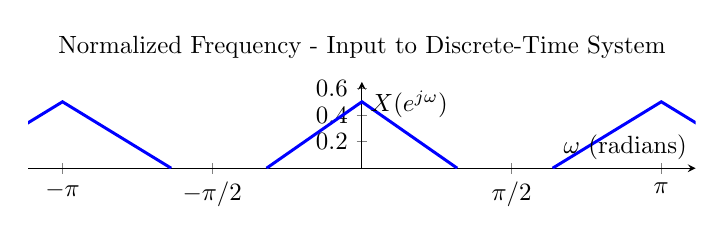
\begin{tikzpicture}[scale=0.9]
    \begin{axis}[
        width=11cm, height=2.8cm,
        xlabel={$\omega$ (radians)},
        ylabel={$X(e^{j\omega})$},
        xmin=-3.5, xmax=3.5,
        ymin=0, ymax=0.65,
        axis lines=middle,
        xtick={-3.14,-1.57,0,1.57,3.14},
        xticklabels={$-\pi$,$-\pi/2$,$0$,$\pi/2$,$\pi$},
        title={Normalized Frequency - Input to Discrete-Time System}
    ]
    \addplot[blue, very thick] coordinates {(-1,0) (0,0.5) (1,0)};
    \addplot[blue, very thick] coordinates {(-4.28,0) (-3.14,0.5) (-2,0)};
    \addplot[blue, very thick] coordinates {(2,0) (3.14,0.5) (4.28,0)};
    \end{axis}
\end{tikzpicture}
\end{center}

\textbf{After Discrete-Time Filtering ($\omega_c < \omega_N$)}:
\begin{center}
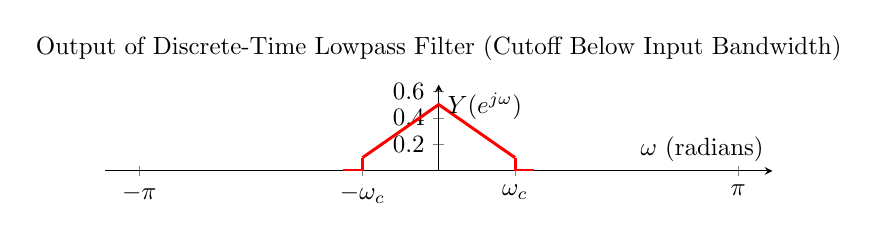
\begin{tikzpicture}[scale=0.9]
    \begin{axis}[
        width=11cm, height=2.8cm,
        xlabel={$\omega$ (radians)},
        ylabel={$Y(e^{j\omega})$},
        xmin=-3.5, xmax=3.5,
        ymin=0, ymax=0.65,
        axis lines=middle,
        xtick={-3.14,-0.8,0,0.8,3.14},
        xticklabels={$-\pi$,$-\omega_c$,$0$,$\omega_c$,$\pi$},
        title={Output of Discrete-Time Lowpass Filter (Cutoff Below Input Bandwidth)}
    ]
    % Filtered output (truncated triangle - trapezoidal shape)
    % The filter cuts off at omega_c = 0.8, which is less than the triangle edge at omega = 1
    % So we need to find the height at omega = 0.8
    % Triangle goes from (0, 0.5) to (1, 0), so at omega = 0.8: height = 0.5 - (0.8/1)*0.5 = 0.5 - 0.4 = 0.1
    \addplot[red, very thick] coordinates {(-0.8,0.1) (-0.8,0) (-1,0)};
    \addplot[red, very thick] coordinates {(-0.8,0.1) (0,0.5) (0.8,0.1)};
    \addplot[red, very thick] coordinates {(0.8,0.1) (0.8,0) (1,0)};
    \end{axis}
\end{tikzpicture}
\end{center}
\end{frame}

\begin{frame}{Relaxed Nyquist Condition}
\textbf{Traditional Nyquist Requirement}:
\[
\Omega_s \geq 2\Omega_N \quad \Rightarrow \quad (2\pi - \Omega_N T) \geq \Omega_N T
\]

\vspace{0.3cm}
\textbf{With Discrete-Time Filtering}:
\[
(2\pi - \Omega_N T) \geq \omega_c
\]

\vspace{0.3cm}
\textbf{Interpretation}:
\begin{itemize}
    \item Can tolerate some aliasing if $H(e^{j\omega})$ removes aliased components
    \item Filter must eliminate frequencies where aliasing occurs
    \item More flexible than strict bandlimiting requirement
    \item Allows lower sampling rates in some applications
\end{itemize}
\end{frame}

\section{Example: Ideal Differentiator}

\begin{frame}{Example: Ideal Bandlimited Differentiator}
\textbf{Continuous-Time Differentiator}:
\[
y_c(t) = \frac{d}{dt}[x_c(t)] \quad \Leftrightarrow \quad H_c(j\Omega) = j\Omega
\]

\vspace{0.3cm}
\textbf{Desired Effective Frequency Response}:
\[
H_{\text{eff}}(j\Omega) = \begin{cases}
j\Omega, & |\Omega| < \pi/T \\
0, & |\Omega| \geq \pi/T
\end{cases}
\]

\begin{center}
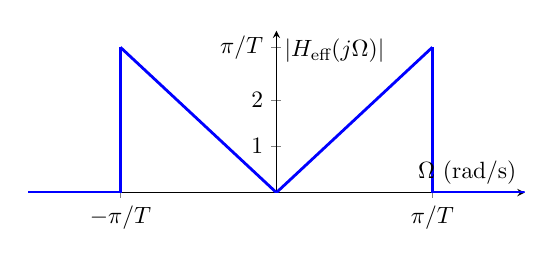
\begin{tikzpicture}[scale=0.85]
  \begin{axis}[
    width=9cm, height=4cm,
    xlabel={$\Omega$ (rad/s)},
    ylabel={$|H_{\text{eff}}(j\Omega)|$},
    xmin=-5, xmax=5,
    ymin=0, ymax=3.5,
    axis lines=middle,
    xtick={-3.1416,0,3.1416},
    xticklabels={$-\pi/T$,$0$,$\pi/T$},
    ytick={0,1,2,3.1416},
    yticklabels={$0$,$1$,$2$,$\pi/T$},
    domain=-5:5
  ]
    % Zero region (left)
    \addplot[blue, very thick] coordinates {(-5,0) (-3.1416,0)};
    % Vertical jump at -pi/T
    \addplot[blue, very thick] coordinates {(-3.1416,0) (-3.1416,3.1416)};
    % Inside passband: |Omega| (left descending to 0 then rising to right edge)
    \addplot[blue, very thick] coordinates {(-3.1416,3.1416) (0,0) (3.1416,3.1416)};
    % Vertical drop at +pi/T
    \addplot[blue, very thick] coordinates {(3.1416,3.1416) (3.1416,0)};
    % Zero region (right)
    \addplot[blue, very thick] coordinates {(3.1416,0) (5,0)};
  \end{axis}
\end{tikzpicture}
\end{center}
\end{frame}

\begin{frame}{Discrete-Time Differentiator Implementation}
\textbf{Required Discrete-Time Frequency Response}:
\[
H(e^{j\omega}) = \frac{j\omega}{T}, \quad |\omega| < \pi
\]

\begin{center}
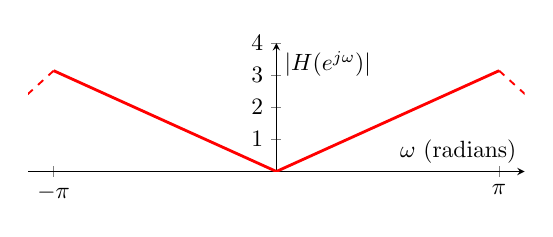
\begin{tikzpicture}[scale=0.85]
    \begin{axis}[
        width=9cm, height=3.5cm,
        xlabel={$\omega$ (radians)},
        ylabel={$|H(e^{j\omega})|$},
        xmin=-3.5, xmax=3.5,
        ymin=0, ymax=4,
        axis lines=middle,
        xtick={-3.14,0,3.14},
        xticklabels={$-\pi$,$0$,$\pi$}
    ]
    % Main period
    \addplot[red, very thick] coordinates {(-3.14,3.14) (0,0) (3.14,3.14)};
    % Periodic extensions (dashed)
    \draw[red, dashed, thick] (axis cs:3.14,3.14) -- (axis cs:4.71,0);
    \draw[red, dashed, thick] (axis cs:-3.14,3.14) -- (axis cs:-4.71,0);
    \end{axis}
\end{tikzpicture}
\end{center}

\textbf{Relationship}: $H(e^{j\omega}) = H_c(j\omega/T)$ (periodic with period $2\pi$)
\end{frame}

\begin{frame}{Impulse Response of Discrete-Time Differentiator}
\textbf{Inverse DTFT}:
\[
h[n] = \frac{1}{2\pi}\int_{-\pi}^{\pi}\frac{j\omega}{T}e^{j\omega n}d\omega
\]

\vspace{0.3cm}
\textbf{Result}:
\[
\boxed{h[n] = \begin{cases}
0, & n = 0 \\
\frac{\cos(\pi n)}{nT}, & n \neq 0
\end{cases}}
\]

\vspace{0.3cm}
\textbf{Properties}:
\begin{itemize}
    \item Non-causal and infinite duration (ideal filter)
    \item Alternating signs: $h[n] = \frac{(-1)^n}{nT}$ for $n \neq 0$
    \item Practical implementation requires windowing and truncation
\end{itemize}
\end{frame}

\section{Impulse Invariance}

\begin{frame}{Impulse Invariance: Time Domain Relationship}
\textbf{Goal}: Given continuous-time system $H_c(j\Omega)$, design discrete-time $H(e^{j\omega})$

\vspace{0.2cm}
\begin{center}
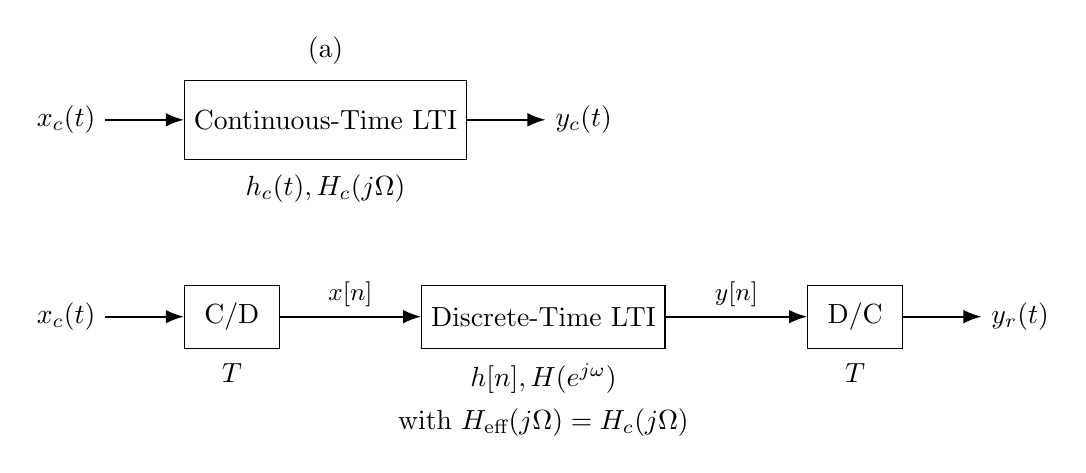
\begin{tikzpicture}[
    >=Latex,
    block/.style={draw, minimum width=3cm, minimum height=1cm, align=center},
    sblock/.style={draw, minimum width=1.2cm, minimum height=0.8cm, align=center},
    tblock/.style={draw, minimum width=2.6cm, minimum height=0.8cm, align=center},
    node distance=1.6cm and 1.6cm
]
    % (a) Continuous-time system
    \node (xin_ct) at (-5.5,1.5) {$x_c(t)$};
    \node[block, right=1.0cm of xin_ct] (ct) {Continuous-Time LTI};
    \node[below=2pt of ct] {$h_c(t), H_c(j\Omega)$};
    \node[right=1.0cm of ct] (yout_ct) {$y_c(t)$};

    \draw[->, thick] (xin_ct) -- (ct.west);
    \draw[->, thick] (ct.east) -- (yout_ct);
    \node[above=2pt of ct] {(a)};

    % (b) Discrete-time equivalent system
    \node (xin_dt) at (-5.5,-1) {$x_c(t)$};
    \node[sblock, right=1.0cm of xin_dt] (cd) {C/D};
    \node[below=2pt of cd] {$T$};

    \node[tblock, right=1.8cm of cd] (dt) {Discrete-Time LTI};
    \node[below=2pt of dt] {$h[n], H(e^{j\omega})$};

    \node[sblock, right=1.8cm of dt] (dc) {D/C};
    \node[below=2pt of dc] {$T$};

    \node[right=1.0cm of dc] (yout_dt) {$y_r(t)$};

    \draw[->, thick] (xin_dt) -- (cd.west);
    \draw[->, thick] (cd.east) -- node[midway, above, font=\small] {$x[n]$} (dt.west);
    \draw[->, thick] (dt.east) -- node[midway, above, font=\small] {$y[n]$} (dc.west);
    \draw[->, thick] (dc.east) -- (yout_dt);

    \node[below=18pt of dt] {with $H_{\text{eff}}(j\Omega) = H_c(j\Omega)$};
\end{tikzpicture}
\end{center}

% \vspace{0.2cm}
% \textbf{Starting Point - Frequency Domain Design}:
% \[
% H(e^{j\omega}) = H_c(j\omega/T), \quad |\omega| < \pi
% \]
% with requirement: $H_c(j\Omega) = 0$ for $|\Omega| \geq \pi/T$
\end{frame}

\begin{frame}{Impulse Invariance: Mathematical Derivation}
\textbf{Step 1 - Apply Sampling Theory}:

Start with sampled impulse response:
\[
h[n] = h_c(nT)
\]

\vspace{0.3cm}
\textbf{Step 2 - Use C/D Frequency Relationship}:

From sampling theory (previous lecture):
\[
H(e^{j\omega}) = \frac{1}{T}\sum_{k=-\infty}^{\infty}H_c\left(j\frac{\omega - 2\pi k}{T}\right)
\]

\vspace{0.3cm}
We are left with periodic replication due to discrete sampling
\end{frame}

\begin{frame}{Impulse Invariance: Deriving the Scale Factor}
\textbf{Step 3 - Apply Bandlimited Condition}:

If $H_c(j\Omega) = 0$ for $|\Omega| \geq \pi/T$, only $k=0$ term survives (Perfect LPF'ing):
\[
H(e^{j\omega}) = \frac{1}{T}H_c\left(j\frac{\omega}{T}\right), \quad |\omega| < \pi
\]

\vspace{0.3cm}
\textbf{Step 4 - Match Desired Response}:

We want: $H(e^{j\omega}) = H_c(j\omega/T)$

But we have: $H(e^{j\omega}) = \frac{1}{T}H_c(j\omega/T)$

\vspace{0.3cm}
\textbf{Solution}: Scale the impulse response by $T$
\[
\boxed{h[n] = Th_c(nT)}
\]

This compensates for the $\frac{1}{T}$ scaling factor in the frequency domain
\end{frame}

\begin{frame}{Impulse Invariance: Final Result}
\textbf{Time Domain Relationship}:
\[
\boxed{h[n] = Th_c(nT)}
\]

\vspace{0.3cm}
\textbf{Frequency Domain Relationship}:
\[
\boxed{H(e^{j\omega}) = H_c(j\omega/T), \quad |\omega| < \pi}
\]

\vspace{0.3cm}
\textbf{Summary of Derivation}:
\begin{enumerate}
    \item Start with sampled impulse response: $h[n] = h_c(nT)$
    \item Apply C/D frequency relationship (periodic replication)
    \item Eliminate aliased terms
    \item Scale by $T$ to match desired frequency response
\end{enumerate}

\end{frame}

\begin{frame}{Impulse Invariance: Ideal Lowpass Example}
\textbf{Continuous-Time Ideal Lowpass}:
\[
H_c(j\Omega) = \begin{cases}
1, & |\Omega| < \Omega_c \\
0, & |\Omega| \geq \Omega_c
\end{cases}, \quad h_c(t) = \frac{\sin(\Omega_c t)}{\pi t}
\]

\vspace{0.3cm}
\textbf{Impulse Invariant Discrete-Time Filter}:
\[
h[n] = Th_c(nT) = T\frac{\sin(\Omega_c nT)}{\pi nT} = \frac{\sin(\omega_c n)}{\pi n}
\]
where $\omega_c = \Omega_c T$

\vspace{0.3cm}
\textbf{Resulting Frequency Response}:
\[
H(e^{j\omega}) = \begin{cases}
1, & |\omega| < \omega_c \\
0, & \omega_c \leq |\omega| \leq \pi
\end{cases}
\]
\end{frame}

\begin{frame}{Impulse Invariance: Suddenly Applied Exponential}
\textbf{Continuous-Time Exponential System}:
\[
h_c(t) = Ae^{s_0 t}u(t) \quad \Leftrightarrow \quad H_c(s) = \frac{A}{s - s_0}, \quad \text{Re}(s) > \text{Re}(s_0)
\]

\vspace{0.3cm}
\textbf{Apply Impulse Invariance}:
\[
h[n] = Th_c(nT) = ATe^{s_0 Tn}u[n]
\]

\vspace{0.3cm}
\textbf{Discrete-Time System Function}:
\[
H(z) = \frac{AT}{1 - e^{s_0 T}z^{-1}}, \quad |z| > |e^{s_0 T}|
\]

\vspace{0.3cm}
\textbf{Frequency Response} (if $\text{Re}(s_0) < 0 \rightarrow \text{stable}$):
\[
H(e^{j\omega}) = \frac{AT}{1 - e^{s_0 T}e^{-j\omega}}
\]
\end{frame}

\begin{frame}{Impulse Invariance: Aliasing Considerations}
\textbf{Exact Relationship Requires}:
\[
H_c(j\Omega) = 0 \text{ for } |\Omega| \geq \pi/T
\]

\vspace{0.3cm}
\textbf{In Practice}:
\begin{itemize}
    \item Most systems are not strictly bandlimited
    \item Aliasing will occur in $H(e^{j\omega})$
    \item Effect may be small if $H_c(j\Omega)$ decays rapidly
\end{itemize}

\vspace{0.3cm}
\textbf{Design Strategy}:
\begin{itemize}
    \item Choose $T$ small enough that $H_c(j\Omega) \approx 0$ for $|\Omega| > \pi/T$
    \item Higher sampling rate reduces aliasing error
    \item Trade-off between computational complexity and accuracy
    \item Impulse invariance is widely used for IIR filter design
\end{itemize}
\end{frame}

\section{Summary}

\begin{frame}{Summary: Key Equations}
\textbf{C/D Conversion}:
\[
x[n] = x_c(nT), \quad X(e^{j\omega}) = \frac{1}{T}\sum_{k=-\infty}^{\infty}X_c\left(j\frac{\omega - 2\pi k}{T}\right)
\]

\textbf{D/C Conversion}:
\[
y_r(t) = \sum_{n=-\infty}^{\infty}y[n]\frac{\sin[\pi(t-nT)/T]}{\pi(t-nT)/T}
\]

\textbf{Effective System}:
\[
H_{\text{eff}}(j\Omega) = \begin{cases}
H(e^{j\Omega T}), & |\Omega| < \pi/T \\
0, & |\Omega| \geq \pi/T
\end{cases}
\]

\textbf{Impulse Invariance}:
\[
h[n] = Th_c(nT), \quad H(e^{j\omega}) = H_c(j\omega/T)
\]
\end{frame}

\begin{frame}{Summary: Design Implications}
\textbf{Advantages of Discrete-Time Processing}:
\begin{itemize}
    \item Programmable filter characteristics
    \item Easily tunable cutoff frequencies (vary $T$, fixed $H(e^{j\omega})$)
    \item Precise, stable implementations (analog systems suffer from variances)
    \item Complex operations (differentiation, filtering) easily realized
\end{itemize}

\vspace{0.3cm}
\textbf{Design Considerations}:
\begin{itemize}
    \item Input must be bandlimited or prefiltered (anti-aliasing filter)
    \item Sampling rate must meet Nyquist (or relaxed) criterion
    \item Aliasing can be tolerated if filtered out by $H(e^{j\omega})$
    \item Impulse invariance is widely used for IIR filter design
\end{itemize}

\vspace{0.3cm}
\textbf{Applications}:
\begin{itemize}
    \item Highly popular in Audio/video processing, communications
    \item Control systems
    \item Any continuous-time signal processing via digital systems
\end{itemize}
\end{frame}

\end{document}